% Options for packages loaded elsewhere
% Options for packages loaded elsewhere
\PassOptionsToPackage{unicode}{hyperref}
\PassOptionsToPackage{hyphens}{url}
%
\documentclass[
  italian,
  letterpaper,
  paper=A4,
  headinclude=on,
  footinclude=on,
  12pt]{scrbook}
\usepackage{xcolor}
\usepackage{amsmath,amssymb}
\setcounter{secnumdepth}{5}
\usepackage{iftex}
\ifPDFTeX
  \usepackage[T1]{fontenc}
  \usepackage[utf8]{inputenc}
  \usepackage{textcomp} % provide euro and other symbols
\else % if luatex or xetex
  \usepackage{unicode-math} % this also loads fontspec
  \defaultfontfeatures{Scale=MatchLowercase}
  \defaultfontfeatures[\rmfamily]{Ligatures=TeX,Scale=1}
\fi
\usepackage{lmodern}
\ifPDFTeX\else
  % xetex/luatex font selection
\fi
% Use upquote if available, for straight quotes in verbatim environments
\IfFileExists{upquote.sty}{\usepackage{upquote}}{}
\IfFileExists{microtype.sty}{% use microtype if available
  \usepackage[]{microtype}
  \UseMicrotypeSet[protrusion]{basicmath} % disable protrusion for tt fonts
}{}
\makeatletter
\@ifundefined{KOMAClassName}{% if non-KOMA class
  \IfFileExists{parskip.sty}{%
    \usepackage{parskip}
  }{% else
    \setlength{\parindent}{0pt}
    \setlength{\parskip}{6pt plus 2pt minus 1pt}}
}{% if KOMA class
  \KOMAoptions{parskip=half}}
\makeatother
% Make \paragraph and \subparagraph free-standing
\makeatletter
\ifx\paragraph\undefined\else
  \let\oldparagraph\paragraph
  \renewcommand{\paragraph}{
    \@ifstar
      \xxxParagraphStar
      \xxxParagraphNoStar
  }
  \newcommand{\xxxParagraphStar}[1]{\oldparagraph*{#1}\mbox{}}
  \newcommand{\xxxParagraphNoStar}[1]{\oldparagraph{#1}\mbox{}}
\fi
\ifx\subparagraph\undefined\else
  \let\oldsubparagraph\subparagraph
  \renewcommand{\subparagraph}{
    \@ifstar
      \xxxSubParagraphStar
      \xxxSubParagraphNoStar
  }
  \newcommand{\xxxSubParagraphStar}[1]{\oldsubparagraph*{#1}\mbox{}}
  \newcommand{\xxxSubParagraphNoStar}[1]{\oldsubparagraph{#1}\mbox{}}
\fi
\makeatother


\usepackage{longtable,booktabs,array}
\usepackage{calc} % for calculating minipage widths
% Correct order of tables after \paragraph or \subparagraph
\usepackage{etoolbox}
\makeatletter
\patchcmd\longtable{\par}{\if@noskipsec\mbox{}\fi\par}{}{}
\makeatother
% Allow footnotes in longtable head/foot
\IfFileExists{footnotehyper.sty}{\usepackage{footnotehyper}}{\usepackage{footnote}}
\makesavenoteenv{longtable}
\usepackage{graphicx}
\makeatletter
\newsavebox\pandoc@box
\newcommand*\pandocbounded[1]{% scales image to fit in text height/width
  \sbox\pandoc@box{#1}%
  \Gscale@div\@tempa{\textheight}{\dimexpr\ht\pandoc@box+\dp\pandoc@box\relax}%
  \Gscale@div\@tempb{\linewidth}{\wd\pandoc@box}%
  \ifdim\@tempb\p@<\@tempa\p@\let\@tempa\@tempb\fi% select the smaller of both
  \ifdim\@tempa\p@<\p@\scalebox{\@tempa}{\usebox\pandoc@box}%
  \else\usebox{\pandoc@box}%
  \fi%
}
% Set default figure placement to htbp
\def\fps@figure{htbp}
\makeatother



\ifLuaTeX
\usepackage[bidi=basic]{babel}
\else
\usepackage[bidi=default]{babel}
\fi
% get rid of language-specific shorthands (see #6817):
\let\LanguageShortHands\languageshorthands
\def\languageshorthands#1{}


\setlength{\emergencystretch}{3em} % prevent overfull lines

\providecommand{\tightlist}{%
  \setlength{\itemsep}{0pt}\setlength{\parskip}{0pt}}



 


\KOMAoptions{DIV=12, BCOR=10mm, headings=standardclasses}
\usepackage{draftwatermark}
\SetWatermarkText{BOZZA}
\SetWatermarkScale{1.5} % bigger/smaller watermark
\SetWatermarkLightness{0.95} % 0=black, 1=white (default 0.8)
\usepackage{datetime}

% set headers and footers
\usepackage{fancyhdr}
\pagestyle{fancy}

% Clear header/foot
\fancyhf{}

% Header: only chapter title (no numbers)
\renewcommand{\chaptermark}[1]{\markboth{#1}{}}
\fancyhead[LE,RO]{\nouppercase{\leftmark}}

% Footer: page numbers left/right depending on page parity
\fancyfoot[LE,RO]{\thepage}

% Custom center footer text
\fancyfoot[C]{\scriptsize \textit{Questo è un libro in fase di scrittura. Ultimo rendering: \today\ \currenttime}. \\ Per aggiornamenti visita: \url{giorgioarcara.github.io/oip-book}}

% Remove numbering and labels from parts
\renewcommand*{\thepart}{} 
\renewcommand*{\partname}{} 
\renewcommand*{\partformat}{}

\usepackage[backend=biber,style=apa]{biblatex}
\addbibresource{references.bib}  % path corretto al tuo .bib
\usepackage{fvextra}
\DefineVerbatimEnvironment{Highlighting}{Verbatim}{breaklines,commandchars=\\\{\}}
%\areaset[0.50in]{4.5in}{8in} uncomment for default Koma option according to template
%\usepackage{fontspec}
%\newfontfamily\headingfont{Alegreya}
\usepackage{pdfpages}
% Redefine \maketitle to do nothing
\renewcommand{\maketitle}{}

% remove table number from captions (to uniform with html)
\usepackage{caption}
% Remove the "Table X:" label for tables (only affects printed captions)
\captionsetup[table]{labelformat=empty, labelsep=none}
\makeatletter
\@ifpackageloaded{bookmark}{}{\usepackage{bookmark}}
\makeatother
\makeatletter
\@ifpackageloaded{caption}{}{\usepackage{caption}}
\AtBeginDocument{%
\ifdefined\contentsname
  \renewcommand*\contentsname{Indice}
\else
  \newcommand\contentsname{Indice}
\fi
\ifdefined\listfigurename
  \renewcommand*\listfigurename{Elenco delle Figure}
\else
  \newcommand\listfigurename{Elenco delle Figure}
\fi
\ifdefined\listtablename
  \renewcommand*\listtablename{Elenco delle Tabelle}
\else
  \newcommand\listtablename{Elenco delle Tabelle}
\fi
\ifdefined\figurename
  \renewcommand*\figurename{Figura}
\else
  \newcommand\figurename{Figura}
\fi
\ifdefined\tablename
  \renewcommand*\tablename{Tabella}
\else
  \newcommand\tablename{Tabella}
\fi
}
\@ifpackageloaded{float}{}{\usepackage{float}}
\floatstyle{ruled}
\@ifundefined{c@chapter}{\newfloat{codelisting}{h}{lop}}{\newfloat{codelisting}{h}{lop}[chapter]}
\floatname{codelisting}{Lista}
\newcommand*\listoflistings{\listof{codelisting}{Elenco degli Elenchi}}
\makeatother
\makeatletter
\makeatother
\makeatletter
\@ifpackageloaded{caption}{}{\usepackage{caption}}
\@ifpackageloaded{subcaption}{}{\usepackage{subcaption}}
\makeatother
\usepackage{bookmark}
\IfFileExists{xurl.sty}{\usepackage{xurl}}{} % add URL line breaks if available
\urlstyle{same}
\hypersetup{
  pdftitle={Oltre i punteggi},
  pdfauthor={Giorgio Arcara},
  pdflang={it},
  hidelinks,
  pdfcreator={LaTeX via pandoc}}


\title{Oltre i punteggi}
\usepackage{etoolbox}
\makeatletter
\providecommand{\subtitle}[1]{% add subtitle to \maketitle
  \apptocmd{\@title}{\par {\large #1 \par}}{}{}
}
\makeatother
\subtitle{Elementi di psicometria e statistica per la neuropsicologia
clinica}
\author{Giorgio Arcara}
\date{2025-09-25}
\begin{document}
\frontmatter
\maketitle

\RecustomVerbatimEnvironment{verbatim}{Verbatim}{
   showspaces = false,
   showtabs = false,
   breaksymbolleft={},
   breaklines
   % Note: setting commandchars=\\\{\} here will cause an error
}

\includepdf[pages=1,fitpaper=true]{Figures/Cover2.pdf}

\renewcommand*\contentsname{Indice}
{
\setcounter{tocdepth}{2}
\tableofcontents
}

\mainmatter
\bookmarksetup{startatroot}

\chapter*{Premesse}\label{premesse}
\addcontentsline{toc}{chapter}{Premesse}

\markboth{Premesse}{Premesse}

\begin{verbatim}
Ultima modifica: 2025-09-25 23:09:19 CEST. Versione 0.1.0
\end{verbatim}

\subsection*{Obiettivo del libro}\label{obiettivo-del-libro}
\addcontentsline{toc}{subsection}{Obiettivo del libro}

Questo libro ha come obiettivo fornire le conoscenze fondamentali di
psicometria e di statistica da utilizzare nella pratica clinica
neuropsicologica. In aggiunta a ciò, il libro contiene sezioni dedicate
alla neuropsicologia forense e alla psicologia clinica in generale. Nel
corso dei suoi capitoli sono trattati diversi aspetti psicometrici e
statistici in una maniera che cerca di essere il più possibile
accessibile e basata su esempi concreti, senza però banalizzare la
complessità degli argomenti trattati. Per le psicologhe e gli psicologi
alle parole ``psicometria'' e ``statistica'' spesso si associano ricordi
dolorosi del periodo universitario piuttosto che aspetti quotidiani
dell'attività professionale. Questo libro ha l'ambizioso obiettivo di
mostrarvi come questo sia profondamente sbagliato e che sia la
psicometria, sia la statistica possano avere un ruolo cruciale
nell'attività clinica.

A differenza di altri testi di psicometria disponibili, il libro si
focalizza specificamente sull' \textbf{applicazione pratica} delle
conoscenze psicometriche e statistiche. Al momento iniziale di scrittura
di questo libro è in programma la scrittura di due volumi, separati ma
strettamente connessi. Il primo (quello presente) è destinato proprio a
chi si occupa di clinica: contiene tutti gli elementi fondamentali, ma
evita approfondimenti relativi alle formule e non scende nei dettagli
più tecnici. Il secondo, più specialistico, sarà sviluppato in un
secondo momento e sarà destinato a chiunque voglia conoscere più in
dettaglio gli aspetti psicometrici e statistici rilevanti per la
neuropsicologia clinica. Quest'ultimo volume sarà dedicato anche a chi
voglia effettuare attività di ricerca nell'ambito e conterrà codice in
\texttt{R} per approfondire gli argomenti esplorati,

\subsection*{Contribuire a questo
libro}\label{contribuire-a-questo-libro}
\addcontentsline{toc}{subsection}{Contribuire a questo libro}

Questo libro è pensato per professioniste/i (principalmente
neuropsicologhe/i cliniche/i e forensi) e idealmente è anche
\emph{sviluppato insieme a loro} in maniera collaborativa. Se hai un
suggerimento su un argomento da trattare, su come migliorare una
spiegazione, se vuoi segnalare un errore di battitura o in generale per
qualsiasi consiglio, puoi usare i pulsanti \emph{``Segnala un
problema''} e \emph{``Modifica questa pagina''} che trovi a destra nella
versione web del libro. In alternativa puoi scrivermi una mail a
\href{mailto:giorgio.arcara@gmail.com}{\nolinkurl{giorgio.arcara@gmail.com}}
. Cercherò di integrare ogni segnalazione/richiesta e il tuo nome verrà
inserito all'interno dei ringraziamenti del libro per riconoscere il tuo
contributo.

\subsection*{Due principi fondamentali}\label{due-principi-fondamentali}
\addcontentsline{toc}{subsection}{Due principi fondamentali}

Ci sono due importanti principi alla base di questo libro che vorrei
esplicitare sin dall'inizio:

\begin{enumerate}
\def\labelenumi{\arabic{enumi}.}
\tightlist
\item
  Le conoscenze psicometriche \emph{possono e dovrebbero} essere
  incorporate nella routine clinica, portando ad un utilizzo più
  consapevole dei test neuropsicologici e psicologici, delle loro
  potenzialità e limiti, e ad interpretazioni più motivate e ragionate.
\item
  Le conoscenze psicometriche \emph{sono solo una parte} delle
  conoscenze necessarie per la pratica clinica. Conoscenze teoriche (es.
  di neuropsicologia cognitiva e clinica) e cliniche (es. su come
  condurre un colloquio) sono altrettanto fondamentali. Questo dovrebbe
  essere scontato, ma è importante chiarire questo punto per una
  corretta lettura del libro e dei suoi contenuti.
\end{enumerate}

\subsection*{Costo del libro (nessuno)}\label{costo-del-libro-nessuno}
\addcontentsline{toc}{subsection}{Costo del libro (nessuno)}

\textbf{Il libro è, e sarà sempre, completamente gratuito}

Tutto il materiale è infatti rilasciato con licenza Creative Commons 4.0
\href{https://creativecommons.org/licenses/by-nc-sa/4.0/deed.it}{CC
BY-NC-SA}.

\includegraphics[width=0.25\linewidth,height=\textheight,keepaspectratio]{Figures/CC_license_3_0.png}

Con questa licenza sei libera/o di scaricare, stampare e distribuire
questa guida. Puoi anche copiare parte dei contenuti e modificarli e
utilizzarli per altri libri o presentazioni, purché sia citata la fonte
di orgine. Al momento della scrittura sto valutando se metterlo anche in
vendita tramite una piattaforma online, ma questo non toglie che la
versione online sarà sempre gratuita. Se utilizzi o distribuisci il
materiale contenuto in questo libro ti prego di utilizzare la seguente
citazione:

\emph{Giorgio Arcara (2025), ``Oltre i punteggi. Elementi di psicometria
e statistica per la neuropsicologia clinica'', rilasciato sotto licenza
CC BY-NC-SA 4.0}

Per alcune informazioni aggiuntive sulle scelte stilistiche/redazionali
guarda la pagina \hyperref[note_redazione]{\textbf{Note di redazione}}.

\vspace{2em}

\subsection*{Indice Provvisorio}\label{indice-provvisorio}
\addcontentsline{toc}{subsection}{Indice Provvisorio}

Di seguito trovi un indice provvisorio del libro. Questo indice potrà
essere modificato sulla base dei commenti ricevuti durante il suo
sviluppo.

\textbf{Introduzione}

\begin{itemize}
\tightlist
\item
  Il protagonista del libro: Il test neuropsicologico
\item
  Il libro in breve
\item
  Una metafora utile
\item
  Cosa il libro NON tratta
\item
  Sezioni speciali: \emph{Approfondimenti}, \emph{Nella pratica
  clinica}, \emph{Errori comuni}
\end{itemize}

\textbf{1. Psicometria per la Neuropsicologia clinica}

\begin{itemize}
\tightlist
\item
  Principi di teoria della misurazione
\item
  I test

  \begin{itemize}
  \tightlist
  \item
    Test di prestazione tipica
  \item
    Test di prestazione massima
  \end{itemize}
\item
  Teoria Classica dei test
\item
  Validità ed Affidabilità

  \begin{itemize}
  \tightlist
  \item
    Tipi di Validità e perché sono importanti
  \end{itemize}
\item
  Affidabilità

  \begin{itemize}
  \tightlist
  \item
    Tipi di affidabilità e perché sono importanti
  \end{itemize}
\item
  Introduzione alla Item Response Theory
\item
  Nella pratica clinica: Come usare Affidabilità e Validità per
  scegliere i test
\item
  Nella pratica clinica: Come usare Affidabilità e Validità per
  interpretare i test
\item
  Errori comuni nel considerare gli aspetti psicometrici dei test
\item
  Capitolo 1: Riassunto
\end{itemize}

\textbf{2. Identificare Deficit e danni cognitivi}

\begin{itemize}
\tightlist
\item
  I concetti di \emph{deficit} e \emph{danno} in valutazione dell'adulto
\item
  Il concetto di \emph{deficit} in età evolutiva
\item
  I dati normativi e il \emph{cut-off di normalità}

  \begin{itemize}
  \tightlist
  \item
    Come si ottengono i dati normativi
  \end{itemize}
\item
  Metodi per calcolare i cut-off di normalità

  \begin{itemize}
  \tightlist
  \item
    Z-score e percentili
  \item
    Metodi basati su regressione

    \begin{itemize}
    \tightlist
    \item
      I Punteggi Equivalenti (Capitani, 1987)
    \item
      Il metodo di Crawford \& Howell (1998) per il caso singolo
    \end{itemize}
  \item
    Altri metodi
  \end{itemize}
\item
  Aspetti importanti da considerare nell'utilizzare i dati normativi
\item
  Nella pratica clinica: esempi di utilizzo dei cut-offs
\item
  Errori comuni nell'utilizzo dei cut-offs di normalità
\item
  Approfondimento: Perché usiamo i cut-off basati su soggetti normali?
\item
  Approfondimento: il MoCA e i problemi della sua introduzione in Italia
\item
  Capitolo 2: Riassunto
\end{itemize}

\textbf{3. Identificare patologie o condizioni di interesse}

\begin{itemize}
\tightlist
\item
  Il \emph{gold standard} in neuropsicologia clinica e forense
\item
  Cut-off di discriminazione
\item
  Sensibilità, Specificità e la curva ROC
\item
  Altre misure di performance di identificazione
\item
  Approfondimento pratico: utilizzare test con cut-off di
  discriminazione
\item
  Errori comuni nell'utilizzo di cut-off di discriminiazione
\item
  Capitolo 3: Riassunto
\end{itemize}

\textbf{4. Indagare cambiamenti nel tempo}

\begin{itemize}
\tightlist
\item
  Affidabilità test-retest e importanza per studiare cambiamenti nel
  tempo
\item
  Forme parallele
\item
  Effetto pratica
\item
  Reliable Change Index e altri metodi per cambiamenti nel tempo
\item
  Errori comuni nell'indagare cambiamenti nel tempo
\item
  Capitolo 4: Riassunto
\end{itemize}

\textbf{5. Confrontare punteggi a test diversi}

\begin{itemize}
\tightlist
\item
  Utilizzo di z-score o percentili.
\item
  Punteggi Equivalenti.
\item
  Capitolo 5: Riassunto
\end{itemize}

\textbf{6. Valutazioni forensi e il problema della Simulazione}

\begin{itemize}
\tightlist
\item
  La validità di performance
\item
  Identificare la simulazione in una valutazione
\item
  Capitolo 6: Riassunto
\end{itemize}

\textbf{7. Il teorema di Bayes e la sua rilevanza in clinica}

\begin{itemize}
\tightlist
\item
  Il teorema di Bayes in breve
\item
  Perché il teorema di Bayes è rilevante in neuropsicologia clinica
\item
  Perché il teorema di Bayes è rilevante in neuropsicologia forense
\item
  Errori comuni: cosa può succedere se non si utilizza il Teorema di
  Bayes nelle interpretazioni.
\item
  Capitolo 7: Riassunto
\end{itemize}

\textbf{8. Interpretare i risultati ai test neuropsicologici}

\begin{itemize}
\tightlist
\item
  Perché \emph{Interpretazione} e non \emph{Lettura}?
\item
  L' \emph{Interpretative Approach} nella pratica clinica
\item
  Esempi di interpretazione

  \begin{itemize}
  \tightlist
  \item
    Interpretare risultati contraddittori ai test
  \item
    Integrare i risultati ai test con informazioni qualitative
  \item
    Interpretare casi anomali
  \end{itemize}
\item
  Conclusioni: il ruolo fondamentale della/del professionista
  nell'utilizzo dei test.
\item
  Capitolo 8: Riassunto
\end{itemize}

\textbf{9. Epistemologia della Neuropsicologia Clinica}

\begin{itemize}
\tightlist
\item
  Perché è importante un capitolo sull'Epistemologia?
\item
  Metodologia ed Epistemologia
\item
  Il potenziale ruolo dell'AI nella valutazione neuropsicologica
\item
  Capitolo 9: Riassunto
\end{itemize}

\textbf{Appendici}

\begin{itemize}
\tightlist
\item
  Note di redazione
\item
  Definizioni
\item
  Registro aggiornamenti
\item
  Statistica di base per la neuropsicologia clinica

  \begin{itemize}
  \tightlist
  \item
    Elementi di probabilità
  \item
    Campione e popolazione (approfondimento)
  \item
    Il concetto di p-value
  \item
    Correlazioni
  \item
    Correlazione e causa
  \item
    Regressioni lineari (in breve)
  \end{itemize}
\end{itemize}

\bookmarksetup{startatroot}

\chapter*{Introduzione}\label{introduzione}
\addcontentsline{toc}{chapter}{Introduzione}

\markboth{Introduzione}{Introduzione}

\section*{Il protagonosta del libro: Il test
neuropsicologico}\label{il-protagonosta-del-libro-il-test-neuropsicologico}
\addcontentsline{toc}{section}{Il protagonosta del libro: Il test
neuropsicologico}

\markright{Il protagonosta del libro: Il test neuropsicologico}

È utile precisare sin da subito che questo volume avrà un protagonista
indiscusso: il \textbf{test neuropsicologico}. Il libro però non sarà,
come ci si potrebbe aspettare, una celebrazione dei test e un continuo
sottolineare su perchè è importante utilizzarli. Dovrete piuttosto
aspettarvi un libro che insegna a capire i \emph{limiti} dei test
neuropsicologici e delle informazioni che ci forniscono. Se da un lato
questo può spaventare (delegare la responsabilità delle conclusioni allo
strumento di misurazione è certamente confortante), il messaggio che se
ne può derivare è in realtà assolutamente positivo per la
professionalità della/del neuropsicologa/o. Quello che penso sia chiaro
emergerà è che il ruolo della/del professionista nell'atto dell'utilizzo
di un test è molto più rilevante di quello che potrebbe sembrare, specie
se si conoscono i principi psicometrici e statistici alla base
dell'utilizzo degli strumenti di misurazione neuropsicologica e
psicologica.

\section*{Il libro in breve}\label{il-libro-in-breve}
\addcontentsline{toc}{section}{Il libro in breve}

\markright{Il libro in breve}

Questo non è un romanzo e non richiede colpi di scena, ed è per questo
ritengo utile fornire sin da subito una panoramica dell'intero contenuto
del libro e della filosofia che lo guida (vedi anche il paragrafo
\hyperref[una-metafora-utile]{una metafora utile}). Il messaggio
principale del testo, e non credo sia sorprendente, è che una solida
conoscenza della psicometria è fondamentale per chi opera nel campo
della neuropsicologia clinica. Questo, e lo sottolineo, non significa
affermare che le valutazioni cliniche e forensi siano incentrate
principalmente sugli aspetti psicometrici; anzi, penso sia vero il
contrario. L'idea che desidero mettere in evidenza è che, \emph{a parità
di competenze cliniche e forensi}, chi possiede una buona padronanza
della psicometria e della statistica sarà in grado di condurre
valutazioni più accurate e rigorose. In aggiunta, avere delle conoscenze
di base di psicometria e statistica per la clinica trattate in questo
libro, contribuisce a ridurre il rischio di errori nell'interpretazione
dei test. Nelle mie interazioni con chi si occupa quotidianamente di
valutazioni cliniche, infatti, un problema che noto spesso è l'
eccessiva fiducia sulle informazioni fornite da un test. Non cercherò
dunque di convincervi che i test sono strumenti obiettivi e cui dovete
affidarvi più a loro che all'occhio clinico. Il mio scopo è invece
quello di mostrare quali sono le informazioni che effettivamente
forniscono i test. Il messaggio è che i risultati ai test non possono
essere meramente \emph{letti} ma vanno e anzi, sono inevitabilmente e
sempre \emph{interpretati}. Che la/il professionista lo voglia oppure
no, metterà sempre qualcosa di proprio nell'utilizzo dei risultati ad un
test e questo è un aspetto fondamentale da tenere in considerazione. In
questo senso, il contenuto del presente libro intreccia conoscenze più
pure di psicometria (che riguardano più la teoria della misurazione e
dei test) o di statistica con quello che è spesso definito come
\emph{``assessment''} e cioè con il procedimento che utilizza
informazioni informazioni dei test e altre informazioni cliniche, come
quelle che provengono da anamnesi o da colloquio, per trarre delle
conclusioni (\cite{chiorri2023teoria}) .

La psicometria e la statistica (si veda il paragrafo
\hyperref[Definizioni]{Definizioni} per un approfondimento) sono utili
essenzialmente in due momenti.

\begin{enumerate}
\def\labelenumi{\arabic{enumi}.}
\tightlist
\item
  Nella scelta dei test da utilizzare (in generale o per una specifica
  valutazione)
\item
  Nell'interpretare il più correttamente possibile i risultati ad uno o
  più test somministrati.
\end{enumerate}

Nel \hyperref[Capitolo-1]{\textbf{Capitolo 1}} il libro tratta elementi
di base di Psicometria. A partire da cosa si intende per
\emph{misurazione} fino alle principali qualità che definiscono la
qualità di un Test e cioè \emph{validità} e \emph{affidabilità}. Usare
un Test in maniera consapevole significa anche conoscere quanto fuziona
bene in quanto strumento di misurazione. Chiunque debba misurare la
temperatura per un sospetto di febbre sa che usare un termometro a
gallio (i termometri a mercurio non esistono più), fornisce una misura
più precisa di utilizzare un termometro digitale da orecchio. Lo stesso
principio dovrebbe valere per i test neuropsicologici, dovremmo sempre
scegliere quelli che hanno le migliori qualità di misura (o conoscerne
quantomeno i loro limiti). Questo influenza le interpretazioni che
possiamo trarne ed è definito in gran parte delle proprietà
psicometriche del test.

Nel \hyperref[Capitolo-2]{\textbf{Capitolo 2}} si parla di uno dei
momenti principali in neuropsicologia forense e clinica e cioè
confrontare il risultato di un test con un valore soglia che ci può
indicare se è presente un \emph{deficit} o un \emph{danno}. Questo
avviene tramite l'utilizzo di \emph{dati normativi}, dati ottenuti da
partecipanti che assumiamo siano ``normali''. Il confronto dei punteggi
con i dati normativi e in particolare con il \emph{cut-off di normalità}
è fondamentale per la neuropsicologia clinica e rappresenta forse il
momento più comune di una valutazione neuropsicologica. Per questa
ragione è un argomento che sarà molto approfondito. Tra gli argomenti
trattati sarà specificato perché è cruciale la differenza tra
\emph{campione} e \emph{popolazione} nell'utilizzo dei dati normativi,
quali sono i limiti di utilizzo di metodi molto diffusi (come gli
\emph{z-scores}) e come valutare la \emph{rappresentatività} dei dati
normativi. Saranno inoltre approfonditi tramite vari esempi pratici come
integrare le conoscenze statistiche approfondite in questo capitolo
nella pratica clinica.

Nel \hyperref[Capitolo-3]{\textbf{Capitolo 3}} vengono trattati quei
test che usano soglie per discriminare un gruppo da un altro, spesso un
gruppo con una patologia nota e un gruppo di partecipanti sani. Sono
approfonditi i modi in cui sono ottenute queste soglie, che chiameremo
\emph{cut-off di discriminazione}. Nel capitolo sono trattati argomenti
comuni nella statistica medica, come \emph{sensibilità},
\emph{specificità} e come utilizzare queste per comprendere le qualità
di un test.

Nel \hyperref[Capitolo-4]{\textbf{Capitolo 4}} è trattato un problema
importantissimo in neuropsicologia clinica e cioò indagare
\emph{cambiamenti nel tempo}: questo è fondamentale per monitorare, per
esempio, se un paziente testato più volte sta effettivamente mostrando
un declino nel tempo oppure se è migliorato in seguito ad un trattamento
riabilitativo. Il capitolo mostra vari metodi possibili per fare questo
e quali sono gli errori più comuni. Il capitolo approfondisce in
particolare uno dei principali problemi che ostacola e influenza le
inferenze che si possono fare da misurazioni ripetute e cioè l'
\emph{effetto pratica}.

Il \hyperref[Capitolo-5]{\textbf{Capitolo 5}} illustra i principali
metodi che permettono di \emph{confrontare i punteggi a test diversi} e
quali sono le principali criticità di questo tipo di confronto.

Il \hyperref[Capitolo-6]{\textbf{Capitolo 6}} è dedicato alla
\emph{neuropsicologia forense} e in particolare all'identificazione di
tentativi di \emph{simulazione} di deficit o danni. Il capitolo tratta i
principali metodi statistici utilizzati per poter identificare un
sospetto simulatore.

Nel \hyperref[Capitolo-7]{\textbf{Capitolo 7}} è fornita una breve
spiegazione di cosa è il \emph{teorema di bayes} e il perché è rilevante
nella pratica clinica. Il capitolo cerca di spiegare in maniera semplice
perché questo teorema matematico è uno dei più importanti mai sviluppato
e perché ogni neuropsicologa o neuropsicologo dovrebbero consocerlo,
quantomeno in maniera intuitiva.

Il \hyperref[Capitolo-8]{\textbf{Capitolo 8}} spiega l'importanza dell'
\emph{interpretazione} dei test, alla luce di tutte le informazioni
disponibili e non solo dei punteggi. IL capitolo spiega inoltre
brevemente cosa è l' \emph{``interpretative approach''} (tr. ``Approccio
interpretativo''), una modalità di integrazione tra clinica e utilizzo
di dati psicometrici proposto da Sara Mondini, Marinella Cappelletti e
me, nel 2022.

Il \hyperref[Capitolo-9]{\textbf{Capitolo 9}} tratta alcuni argomenti
che ritengo necessario inserire in un testo di questo genere e che
affrontano temi delicati, che per motivi di spazio saranno soltanto
trattati in superficie. Il primo paragrafo spiega perché è importante
l'epistemologia della neuropsicologia clinica e come una mancanza di un
accordo comune su certi base epistemologiche è, almeno in parte, un
grosso freno allo sviluppo della neuropsicologia clinica stessa. Il
secondo approfondisce la relazione (e differenza), tra metodologia ed
epistemologia. Un paragrafo è dedicato al tema scottante
dell'intelligenza artificiale e fornisce alcuni spunti su come può
essere utilizzata in maniera virtuosa nell'ambito di applicazione di
aspetti psicometrici e statistici in clinica.

Il libro contiene anche diverse \textbf{Appendici}: la prima chiarisce
alcune scelte redazionali, la seconda chiarisce alcuni scelte
metodologiche ed epistemologiche del libro ed elenca in dettaglio le
definizioni di alcuni termini tecnici utilizzati. L'ultima contiene
degli approfondimenti di statistica di base, utili per chi volesse
ripassarle.

\section*{Una metafora utile}\label{una-metafora-utile}
\addcontentsline{toc}{section}{Una metafora utile}

\markright{Una metafora utile}

Per spiegare la filosofia alla base di questo libro utilizzerò una
metafora a cui sono affezionato e che è stata utilizzata da Harald
Baayen (Professore di Linguistica Quantitativa all'Università di
Tubingen) durante un corso di statistica a cui ho avuto la fortuna di
partecipare nel 2008 ad Edmonton, in Canada\footnote{Resta inteso che
  potrei avere un ricordo distorto della citazione, per cui mi prendo
  eventuali responsabilità in caso di inesattezze.}. Il corso era di
statistica per linguisti e psicolinguisti, ma si applica benissimo a
qualsiasi utilizzatore di statistica e, nel nostro caso, anche di
psicometria. Non ricordo esattamente le parole, ma il concetto era il
seguente:

\emph{``utilizzare la statistica è come guidare un'automobile, non
occorre capire come funziona il motore per utilizzarla bene, basta
sapere cosa è giusto o cosa non è giusto fare.''}

\begin{figure}[H]

{\centering \includegraphics[width=0.5\linewidth,height=\textheight,keepaspectratio]{chapters/../Figures/Auto_ChatGPT_BN.png}

}

\caption{\textbf{Utilizzare i test come guidare un automobile}: non
serve conoscere il funzionamento esatto del motore per poterla guidare
in maniera adeguata (ma vedi la prossima Figura)}

\end{figure}%

Detta da H. Baayen, grandissimo esperto di statistica, questa
affermazione faceva sorridere gli studenti, ma era chiara: utilizzare i
metodi statistici correttamente non implica necessariamente conoscere
tutto ciò che sta al di sotto, ma capire cosa è corretto fare e cosa non
è corretto fare. Nel corso degli anni ho però pensato che fosse utile
aggiungere una seconda parte che la metafora in un certo senso, già
implica.

\emph{``è vero che non serve conoscere come funziona il motore di
un'automobile per saperla guidare, ma chi conosce bene come funziona il
motore permette di sfruttarne meglio le potenzialità. Questo è ciò che
accade per esempio per i piloti di formula 1''}

\begin{figure}[H]

{\centering \includegraphics[width=0.4\linewidth,height=\textheight,keepaspectratio]{chapters/../Figures/F1_1_ChatGPT_BN.png}

}

\caption{\textbf{Guidare un auto di F1 }: per essere un pilota
professionista occorre conoscere bene come funziona il motore della
propria vettura (ma guarda la prossima figura)}

\end{figure}%

Per tornare al nostro argomento (e cioè i metodi statistici per la
neuropsicologia) già conoscere cosa è corretto e cosa è sbagliato fare
in termini di utilizzo dei test in neuropsicologia clinica e forense è
molto importante, ma una conoscenza più approfondita ci permette di
utilizzarli meglio e di capire in quali situazioni ci possono essere
problemi o situazioni particolari che meritano attenzione.

Nello scrivere questo libro ho realizzato che si puà aggiungere una
terza parte alla metafora che mi sembra particolarmente pertinente.

\emph{``un pilota non è però un ingegnere o un meccanico che è in grado
di montare e smontare un motore o addirittura di costruirlo. Ne conosce
bene il funzionamento (più di una persona comune), per notare possibili
problemi, come vibrazioni o rumori insoliti e aiutare a comunicare con
il team, ma rimane pur sempre un utilizzatore, che deve concentrarsi su
altre abilità, cioè quelle di guida''}

\begin{figure}[H]

{\centering \includegraphics[width=0.4\linewidth,height=\textheight,keepaspectratio]{chapters/../Figures/Mechanic_ChatGPT_BN.png}

}

\caption{\textbf{Un pilota di F1 ha comunque una conoscenza limitata del
funzionamento del motore}: non possiede necessariamente le competenze di
un meccanico o di un ingegnere, e questo è del tutto normale, non è ciò
che ci si aspetta da chi guida a livello professionistico}

\end{figure}%

\emph{In conclusione}

La metafora che ho qui illustrato mi è utile a chiarire il \emph{perché}
è importante conoscere la psicometria per la pratica in neuropsicologia
clinica e forense. Alcune conoscenze di base sono fondamentali per poter
utilizzare correttamente i nostri strumenti senza fare errori (nella
metafora sarebbe come usare l'acceleratore per frenare). Conoscere
meglio il funzionamento dei test ci permette di capire quali sono i loro
limiti, specie in situazioni non convenzionali (es. posso utilizzare il
mio test se l'età del mio paziente non è rappresentata nel campione
normativo?). Non tutti dobbiamo però essere ``ingegneri'' dei test: non
penso affatto sia necessario che per utilizzare in maniera corretta i
test sia necessario o imprescindibile conoscere ogni dettaglio tecnico e
statistico dello sviluppo. Del resto ci sono specialisti che si occupano
di questo. Questo è ciò che normalmente accade in ogni branca clinica o
applicativa in cui ci sia utilizzo di strumenti, anche di alta
precisione, non è necessario conoscerne ogni dettaglio per poterli usare
efficacemente.

\section*{Cosa il libro NON tratta}\label{cosa-il-libro-non-tratta}
\addcontentsline{toc}{section}{Cosa il libro NON tratta}

\markright{Cosa il libro NON tratta}

La guida è essenzialmente focalizzata su utilizzo dei test e quindi su:
proprietà psicometriche dei test e quella analisi riferite al caso
singolo. Non tratta analisi di gruppi di pazienti perché meno rilevante
per la neuropsicologia clinica e forense, nella loro pratica
professionale. Non tratta inoltra di alcuni aspetti
metodologico/statistici fondamentali per la \emph{neuropsicologia
cognitiva} perché non sono direttamente rilevanti per la pratica clinica
(es. la doppia dissociazione, che implica il confronto di due pazienti
con deficit ``puri'' e che è rilevante per inferenze teoriche, ma meno
per la pratica clinica di una/o neuropsicologa/o). Il libro tratta solo
in maniera marginale gli aspetti dell'Assessment che forniscono
informazioni fondementali per una buona valutazione clinica o forense,
come l'anamnesi e il colloquio. In generale non fornisce informazioni su
come condurre in maniera appropriata queste fasi perché di pertinenza
più clinica che non psicometrico/statistica. Parte di queste
informazioni aggiuntive sono trattate in altri libri a cui ho
contribuito
(\cite{mondini2009valutazione,mondini2016semeiotica,mondini2022methodology})

\section*{\texorpdfstring{Sezioni speciali: \emph{Approfondimenti e
curiosità}, \emph{Nella pratica clinica}, \emph{Errori
comuni}}{Sezioni speciali: Approfondimenti e curiosità, Nella pratica clinica, Errori comuni}}\label{sezioni-speciali-approfondimenti-e-curiosituxe0-nella-pratica-clinica-errori-comuni}
\addcontentsline{toc}{section}{Sezioni speciali: \emph{Approfondimenti e
curiosità}, \emph{Nella pratica clinica}, \emph{Errori comuni}}

\markright{Sezioni speciali: \emph{Approfondimenti e curiosità},
\emph{Nella pratica clinica}, \emph{Errori comuni}}

Per facilitare la comprensione di certi concetti il volume contiene
delle sezioni speciali che hanno come scopo il trattamento più
dettagliato di alcuni aspetti.

\begin{itemize}
\tightlist
\item
  Le sezioni \emph{``Nella pratica clinica''}, illustrano applicazioni
  pratiche dei concetti spiegati, fornendo esempi concreti.
\item
  Le sezioni \emph{``Errori comuni''}, hanno lo scopo di rafforzare
  alcuni concetti utilizzando una prospettiva diversa: invece di dire
  cosa sarebbe corretto fare, sottolineano quali sono degli errori
  comuni, fornendo motivazioni dettagliate del perché certi
  comportamenti sarebbero da considerare appunto errori.
\item
  Le sezioni \emph{``Approfondimenti e cuoriosità''}, come il titolo
  suggerisce, forniscono un trattamento più dettagliato di alcuni
  argomenti o curiosità storiche, teoriche, tecniche, o di altro tipo.
\end{itemize}

\bookmarksetup{startatroot}

\chapter{Psicometria per la neuropsicologia
clinica}\label{psicometria-per-la-neuropsicologia-clinica}

\section{Valutazioni neuropsicologiche, test e misurazione: una
riflessione
iniziale}\label{valutazioni-neuropsicologiche-test-e-misurazione-una-riflessione-iniziale}

Quando si parla di ``valutazione neuropsicologica'', la prima cosa che
viene in mente è certamente una persona che sta effettuando una serie di
test per riuscire a comprendere lo stato cognitivo di un individuo. Lo
scopo potrebbe essere l'accertamento sul sospetto di una patologia in
corso (es. un sospetto di demenza), o la caratterizzazione di un
disturbo cognitivo in una condizione accertata (es. capire se un trauma
cranico ha avuto delle conseguenze). Le informazioni possono avere fini
diagnostici, prognostici o riabilitativi. Quello che accomuna tutti
questi scenari è che difficilmente ci si potrebbe immaginare una
valutazione neuropsicologica completamente senza test e, aggiungo, senza
l'utilizzo di punteggi. Immaginiamo di voler descrivere a qualcuno che
deve sottoporsi ad una valutazione neuropsicologica e che non sa ancora
in cosa consiste, la risposta potrebbe essere qualcosa del tipo \emph{''
le verranno fatto alcune domande e verranno somministrate alcune prove,
ad esempio ricordare una lista di parole, o fare altri semplici compiti.
Alla fine tutte queste informazioni saranno utilizzate per capire come
funziona la tua mente o, più precisamente, i suoi processi cognitivi.''}
Provando a chiedere a ChatGPT4.0 la seguente cosa \emph{Crea un disegno
in bianco e nero di una neuropsicologa che sta effettuando una
valutazione neuropsicologica} il risultato che ho ottenuto (14/09/2025)
è la figura qui di seguito.

\begin{figure}[H]

{\centering 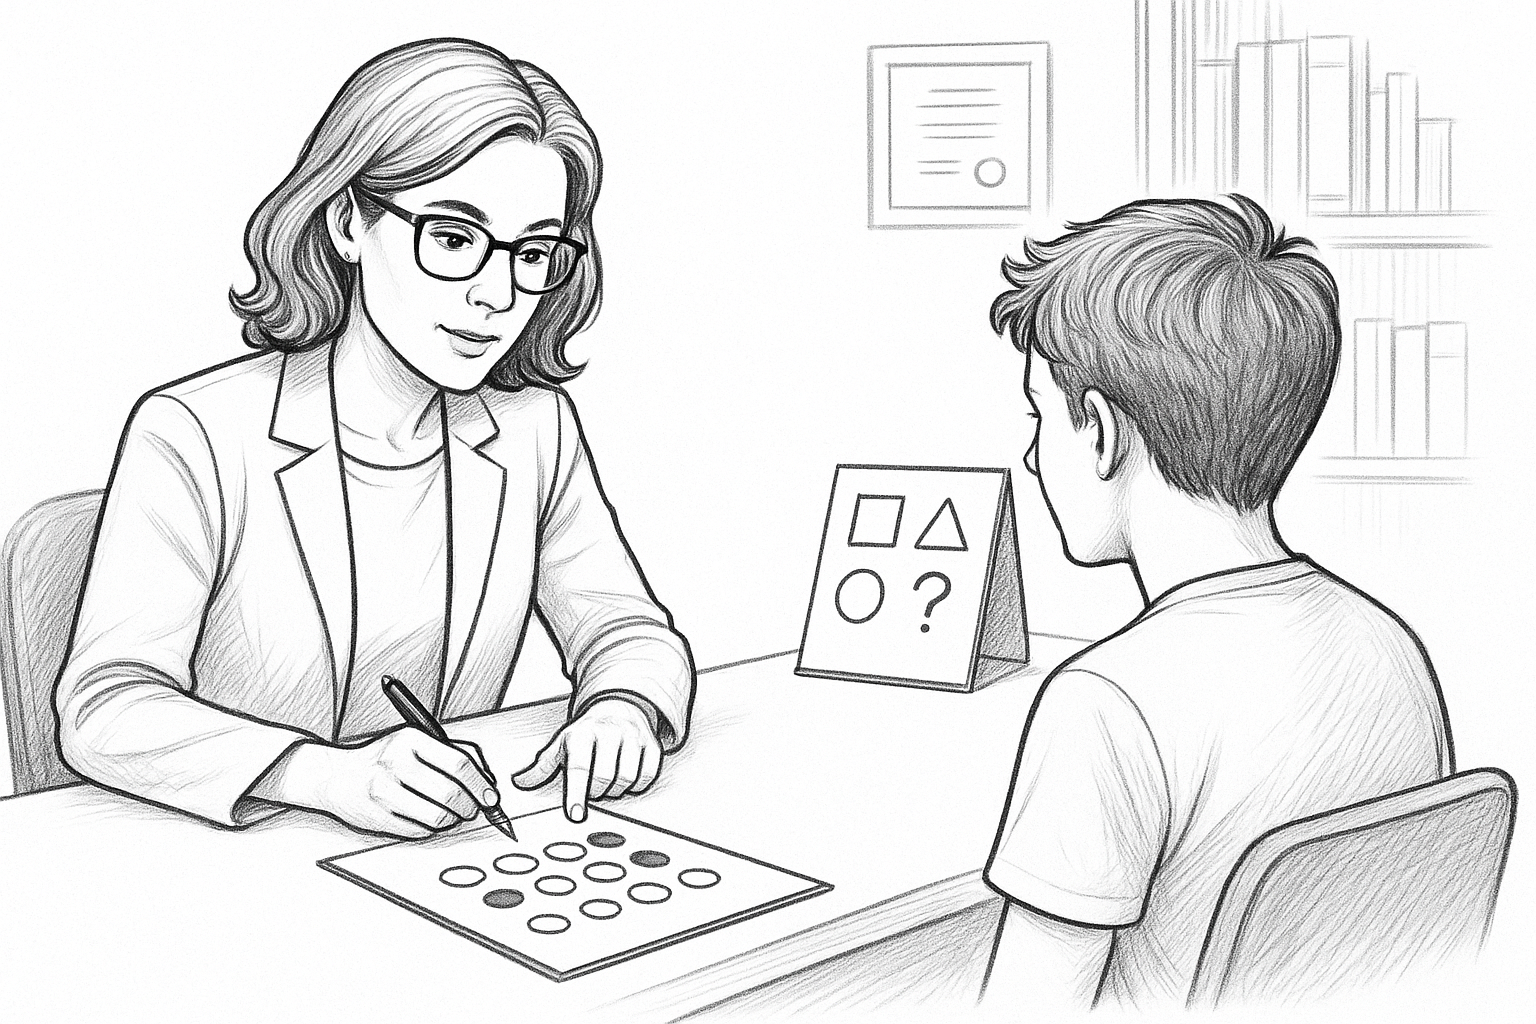
\includegraphics[width=0.6\linewidth,height=\textheight,keepaspectratio]{chapters/../Figures/Valutazione_Neuropsi_ChatGPT.png}

}

\caption{Una valutazione neuropsicologica secondo ChatGPT (vedi testo
per il prompt esatto)}

\end{figure}%

La figura (come siamo abituati adesso con questi sistemi di
``Intelligenza Artificiale'') è piuttosto accurata e quello che mostra è
proprio una persona che somministra un \textbf{test} (vedi
\hyperref[i-test]{prossimo paragrafo}.

Tutta questa premessa (un po' ridondante), serve unicamente a chiarire
che la neuropsicologia clinica è intrinsecamente legata alla
somministrazione dei test sullo stato cognitivo, tanto che le cose sono
spesso considerate inscindibili. Non solo, la valutazione
neuropsicologica fa praticamente sempre utilizzo di \emph{punteggi} dei
test (cioè numeri) per trarre delle conclusioni. I punteggi sono
confrontati con delle soglie e se i valori sono al di là di queste
soglie, viene concluso che qualcosa probabilmente non va (useremo più
avanti termini più tecnici e definizioni più precise). La persona con il
punteggio al di là della soglia potrebbe avere un deficit cognitivo, o
forse un rischio di avere una patologia neurodegenerativa. Va da sé, che
se questa è di norma la pratica neuropsicologica clinica, come
utilizziamo questi punteggi (cioè dei numeri), come li confrontiamo con
queste soglie (chiamate ``cut-off'') è fondamentale perché rappresenta
una parte fondante proprio della pratica clinica. Nel \textbf{prossimo
paragrafo} vedremo come l'utilizzo di punteggi non è altro che un caso
di \emph{misurazione} .

La disciplina che si occupa della misurazione in psicologia (e in
neuropsicologia) è la \emph{psicometria}, una delle materie insieme alla
statistica, che rappresentano le fondamenta di questo libro. La
psicometria si occupa proprio delle questioni della misurazione in
psicologia, una tipologia di misurazione molto particolare perchè non
tratta di proprietà di oggetti fisici ma di concetti psicologici. Una
caratteristica peculiare della misurazione psicologica è che la
relazione tra ciò che è l'esito della misura (cioè il punteggio) e ciò
che si vuole misurare, cioè il costrutto è molto indiretto. Il fatto che
ci sia un'intera disciplina dedicato a questo sottolinea una cosa
importante: la misurazione in psicologia è un argomento complesso che
non può essere banalizzato o trascurato.

Immaginate di dover fare un esame del sangue per capire se avete qualche
anomalia che potrebbe segnalare una patologia. Immaginate adesso di
poter scegliere tra due centri: Il primo utilizza una nuova tecnologia
all'avanguardia, che porta a risultati molto precisi. Il secondo
utilizza invece una tecnologia degli anni 70, notoriamente imprecisa.
Quale centro scegliereste? Immagino che la scelta ricadrebbe sul centro
con lo strumento più moderno e preciso. Ma complichiamo l'esempio:
supponiamo adesso che sappiate che nel centro con lo strumento più
moderno i tecnici e i medici che si occupano dello strumento non godano
di una buona fama ed è noto non conoscano bene l'utilizzo di questo
strumento innovativo. Immaginate inoltre, che nel centro con la
tecnologia obsoleta il medico di riferimento sia un luminare, esperto
della patologia che state indagando. Quale scegliereste? In questo caso
la scelta è certamente più difficile. Ed è giusto che sia così: gli
strumenti di misurazione non sono tutto e la capacità clinica, in questo
caso del medico, va certamente considerata. Se non fosse altrimenti
sceglieremmo principalmente sulla base dello strumento e non del medico.
Spero che però sia chiaro quale vuole essere il mio punto e l'analogia
che voglio sottolineare: i test non sono certamente la sola cosa
importante in una valutazione ma, \emph{in quanto strumenti di
misurazione}, possono essere più o meno precisi e possono essere usati
più o meno correttamente. Immaginate i quattro scenari descritti nella
tabella sotto che corrispondono a quattro centri clinici (A, B, C e D),
Quale centro scegliereste?

\begingroup
{\footnotesize

\begin{longtable}[]{@{}
  >{\centering\arraybackslash}p{(\linewidth - 4\tabcolsep) * \real{0.3750}}
  >{\centering\arraybackslash}p{(\linewidth - 4\tabcolsep) * \real{0.3529}}
  >{\centering\arraybackslash}p{(\linewidth - 4\tabcolsep) * \real{0.2721}}@{}}
\caption{Tabella 1.1: Quattro diversi centri clinici tra cui
scegliere.}\tabularnewline
\toprule\noalign{}
\begin{minipage}[b]{\linewidth}\centering
\end{minipage} & \begin{minipage}[b]{\linewidth}\centering
\textbf{Strumento preciso/ usato bene }
\end{minipage} & \begin{minipage}[b]{\linewidth}\centering
\textbf{Strumento impreciso/ usato male}
\end{minipage} \\
\midrule\noalign{}
\endfirsthead
\toprule\noalign{}
\begin{minipage}[b]{\linewidth}\centering
\end{minipage} & \begin{minipage}[b]{\linewidth}\centering
\textbf{Strumento preciso/ usato bene }
\end{minipage} & \begin{minipage}[b]{\linewidth}\centering
\textbf{Strumento impreciso/ usato male}
\end{minipage} \\
\midrule\noalign{}
\endhead
\bottomrule\noalign{}
\endlastfoot
\textbf{Personale clinico esperto} & Centro A & Centro B \\
\textbf{Personale clinico non esperto} & Centro C & Centro D \\
\end{longtable}

}
\endgroup

Penso che chiunque e senza dubbi, se potesse scegliere a parità di altre
condizioni tra questi centri, sceglierebbe il Centro A. Ho usato questo
stratagemma retorico per chiarire un principio di base e la sua
motivazione: utilizzare strumenti precisi e utilizzarli bene è
fondamentale, ma non è certamente tutto. Le competenze cliniche in
alcuni casi possono anche sopperire in maniera importante eventuali
carenze nell'utilizzo dei test e dei punteggi. A parità però di
competenze cliniche, tutti sceglieremmo chi utilizza i test migliori e
nella maniera più appropriata. È importante sottolineare che
nell'esempio sopra non si parla soltanto di usare strumenti accurati, ma
anche di \emph{saperli usare correttamente}. Questo è un piccolo
dettaglio con implicazioni molto importanti (e che saranno trattate
ampiamente nel libro). Non si tratta solo di scegliere i test migliori,
ma anche di usarli nella maniera più appropriata. In sostanza, conoscere
la psicometria e la statistica per chi fa neuropsicologia dovrebbe avere
lo scopo finale di effettuare valutazioni migliori. Non voglio però
suggerire che sia utile o importante fare confronti tra professioniste e
professionisti in una sorta di competizione. Il confronto dovrebbe
essere piuttosto con se stessi: poiché l'utilizzo dei test e misurazione
sono così importanti nella neuropsicologia clinica, usare i test
migliori e utilizzarli nel modo più corretto può essere la chiave per
diventare diventare una \emph{versione migliore di sè stessi, in quanto
professionisti}.

Queste considerazioni però aprono tanti altri quesiti a cui diventa
importante rispondere. Come fare a capire quali test sono più precisi o,
in generale, migliori per poterli utilizzare? Come utilizzare
correttamente i numeri e le classificazioni che risultano dai risultati
ai test? Risponderemo a tutte queste domande nel corso di questo libro.
Il percorso non sarà breve e per farlo dobbiamo partire proprio dalle
basi e cioè su cosa significa misurare.

\section{Misurazione e neuropsicologia
clinica}\label{misurazione-e-neuropsicologia-clinica}

Il più delle volte in neuropsicologia somministriamo test per ottenere
dei punteggi e cioè dei numeri. Questi numeri ci aiutano a descrivere
ciò che è di interesse che, il più delle volte è legato
\textbf{costrutti neuropsicologici, psicologici o cognitivi}, quali
memoria, attenzione, benessere, depressione, etc. L'utilizzo dei numeri
ci aiuta a capire meglio il funzionamento cognitivo cognitivo e capire
se, per esempio, per una specifica funzione (es. la memoria) è talmente
basso da farci sospettare un deficit oppure l'inizio di una patologia
neurodegenerativa. Allo stesso tempo l'avere dei numeri ci permette di
avere una stima della capacità in un certo momento per poi tornare ad
ripetere la rilevazione e vedere se c'è stato un peggioramento, per
esempio dovuto ad un declino, oppure un miglioramento, per esempio
dovuto ad un trattamento riabilitativo.\\
Ciò che abbiamo descritto sopra non è altro che esempi di
\emph{misurazione} di una proprietà del funzionamento mentale: tramite i
test misuriamo la memoria, misuriamo l'attenzione o altre
caratteristiche di interesse. Per una trattazione approfondita diventa
però necessario dare una definizione di cosa si intenda esattamente per
\emph{misurare} e già qui sorgono i primi problemi. Non esiste infatti
una definizione di misurazione unanimamente accettata (questa
considerazione sarà proprio il punto di partenza del paragrafo
\hyperref[introduzione-item-response-theory]{Introduzione all'Item
Response Theory}). Esistono però delle definizioni molto diffuse, s e
alcune di queste sono implicitamente utilizzate in maniera molto diffusa
nella neuropsicologica clinica. La più famosa definizione di misurazione
è certamente quella di S.S. Stevens, che in un articolo del 1946 ha
fornito una definizione che influenzato (nel bene e nel male) la storia
della psicologia (\cite{stevens1946measurement}) :

\emph{``\ldots possiamo dire che la misurazione, nel senso piu ampio, è
definita come l'assegnazione di numeri a oggetti o eventi secondo
determinate regole.'' (p.~667) }

La proposta di Stevens va contestualizzata al clima del momento. Alla
fine degli anni 40 si stava discutendo (in ambito scientifico), se gli
oggetti di interesse della psicologia potessero essere misurati e se,
quindi, la psicologia potesse essere considerata una scienza. L'iniziale
conclusione di una commissione internazionale di fisici e psicologi che
si era riunita per dare una risposta a questa domanda era arrivata alla
conclusione che, secondo una definizione rigorosa di misurazione, la
risposta era \emph{no}. Secondo Stevens però, il problema era proprio
nei presupposti della commissione e, più in particolare, nella
definizione troppo restrittiva di misurazione. Propose dunque la
definizione riportata sopra, e sottolineò che anche se ogni regola porta
a misurazione, un aspetto importante (ma separabile) è l'utilizzo che si
può fare dei numeri o classificazioni e questo dipende dalla
\textbf{Scala di Misurazione}. A seconda delle proprietà misurate (ma
che possiamo sempre definire come una \emph{misurazione} ) potrebbe
quindi essere diverso l'utilizzo che possiamo fare dei numeri. Per
esempio, il solo rilevare se una persona è femmina o maschio è, secondo
la definizione di Stevens, un caso di misurazione e la scala
utilizzabile sarebbe una \emph{scala categoriale}. In questo caso non
hanno senso operazioni tipo addizione o sottrazione o moltiplicazione
(non ha senso dire che una femmina è due volte un maschio o viceversa) e
una delle poche operazioni possibili è contare quanti casi abbiamo per
ogni categoria (es. confrontare il numero di femmine con il numero di
maschi). Un riassunto delle scale e delle operazioni possibili è
riportata nella tabella 1.2. La proposta di Stevens salvava la
psicologia come scienza e anzi aiutava a chiarire l'utilizzo dei numeri
per la misurazione in diverse circostanze.

\begingroup
{\scriptsize

\begin{longtable}[]{@{}
  >{\raggedright\arraybackslash}p{(\linewidth - 6\tabcolsep) * \real{0.0773}}
  >{\raggedright\arraybackslash}p{(\linewidth - 6\tabcolsep) * \real{0.4309}}
  >{\raggedright\arraybackslash}p{(\linewidth - 6\tabcolsep) * \real{0.1823}}
  >{\raggedright\arraybackslash}p{(\linewidth - 6\tabcolsep) * \real{0.3094}}@{}}
\caption{Tabella 1.2: Le quattro tipologie di scale di misurazione
secondo S.S. Stevens.}\tabularnewline
\toprule\noalign{}
\begin{minipage}[b]{\linewidth}\raggedright
Scala
\end{minipage} & \begin{minipage}[b]{\linewidth}\raggedright
Descrizione
\end{minipage} & \begin{minipage}[b]{\linewidth}\raggedright
Esempio
\end{minipage} & \begin{minipage}[b]{\linewidth}\raggedright
Operazioni possibili
\end{minipage} \\
\midrule\noalign{}
\endfirsthead
\toprule\noalign{}
\begin{minipage}[b]{\linewidth}\raggedright
Scala
\end{minipage} & \begin{minipage}[b]{\linewidth}\raggedright
Descrizione
\end{minipage} & \begin{minipage}[b]{\linewidth}\raggedright
Esempio
\end{minipage} & \begin{minipage}[b]{\linewidth}\raggedright
Operazioni possibili
\end{minipage} \\
\midrule\noalign{}
\endhead
\bottomrule\noalign{}
\endlastfoot
\textbf{Nominale} & Classificazione in categorie senza ordine implicito
& Sesso (M/F), Colori, Nazionalità & Conteggio, moda, verifica
uguaglianza/differenza \\
\textbf{Ordinale} & Classificazione con ordine, ma le distanza tra
categorie non hanno significato & Posizione in una classifica, Titolo di
studio & Ordinamento, mediane, percentili \\
\textbf{Intervallo} & Misura con ordine e intervalli uguali, ma senza
zero assoluto significativo & Temperatura in °C, IQ & Addizione,
Sottrazione,Media, Deviazione standard, z-score \\
\textbf{Rapporto} & Misura con ordine, intervalli uguali e lo zero ha un
significato & Età, Scolarità in anni, tempi di reazione & Tutte le
operazioni aritmetiche (×, ÷, +, −), z-score, rapporti \\
\end{longtable}

\textbf{Legenda}\\
- \emph{Scala}: tipo di misura secondo la classificazione di Stevens.\\
- \emph{Descrizione}: caratteristiche principali della scala.\\
- \emph{Esempio}: variabili reali che rientrano in quella scala.\\
- \emph{Operazioni possibili}: trasformazioni matematiche e statistiche
consentite dai dati.

}
\endgroup

Adesso proviamo però ad andare oltre alla definizione di Stevens e
approfondire ulteriormente il significato di misurazione. In generale
misurare significa utilizzare numeri per descrivere delle proprietà di
entità che vogliamo descrivere. Ad esempio quando misuriamo la lunghezza
di un tavolo, supponendo che essa sia 50 cm, il numero ``50'' indica una
proporietà del tavolo in una maniera per noi utile. Definiamo qui il
\emph{Sistema Relazionale Empirico}, come l'insieme di entità del mondo
empirico che hanno una determinata proprietà che vogliamo misurare (es.
oggetti di diversa lunghezza) e il \emph{Sistema Relazionale Numerico}
un insieme di numeri (es. i numeri Reali) con i quali vogliamo
descrivere questa misura.

\begin{center}
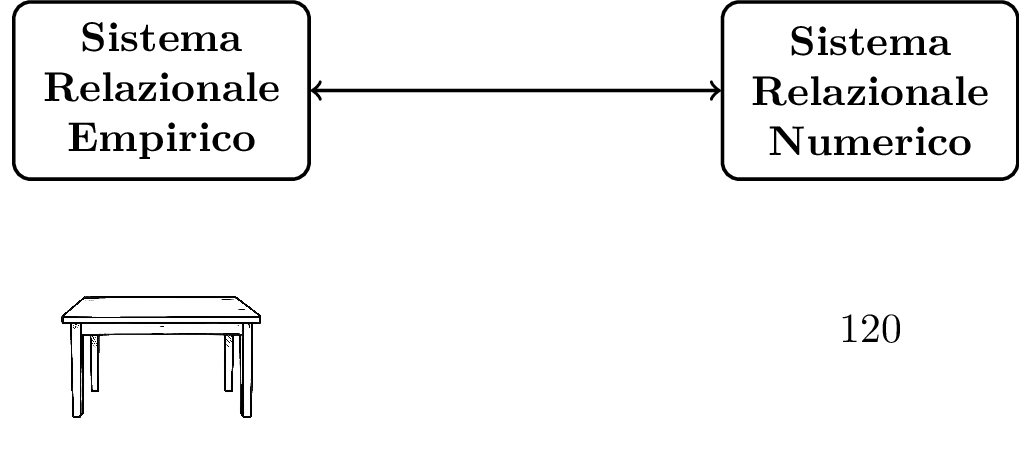
\includegraphics[width=0.7\linewidth,height=\textheight,keepaspectratio]{chapters/../Figures/Latex - Figure Measurement 1/Fig_measurement_1.png}
\end{center}

Nell'esempio della Figura sopra, un tavolo ha un lato lungo 120 cm.
Possiamo usare questo numero (120) per numerosi utilizzi. Supponiamo ad
esempio di avere due tavoli quadrati, uno con il lato di 120 cm e uno
con il lato di 60 cm. Tramite questa misurazione del loro lato, sappiamo
che il tavolo con lato 120 cm è più lungo di quello con lato 60 cm.
Sappiamo che il tavolo con lato 120 cm ha il lato di 60 cm più lungo di
quello con lato 60 cm. Infine sappiamo che il tavolo con lato 120 cm è
lungo il doppio del tavolo con lato 60 cm (nello stesso spazio del
tavolo lungo 120 cm, possiamo mettere due tavoli da 60 cm). Questi
numeri ci permettono dunque di una serie di operazioni utili per
comprendere le proprietà dei tavoli, in questo caso la loro lunghezza, e
interagire con loro. Tornando alla Tabella 1.2, La lunghezza di un
tavolo è misurata su una \emph{scala a rapporti} e sapere questo ci
permette di sapere quali operazioni possiamo fare con i numeri associati
alla misura. La stessa cosa accade quando vogliamo fare una misurazione
psicologica o neuropsicologica. Lo scopo è ottenere un numero che
vogliamo utilizzare per alcuni scopi.

\begin{center}
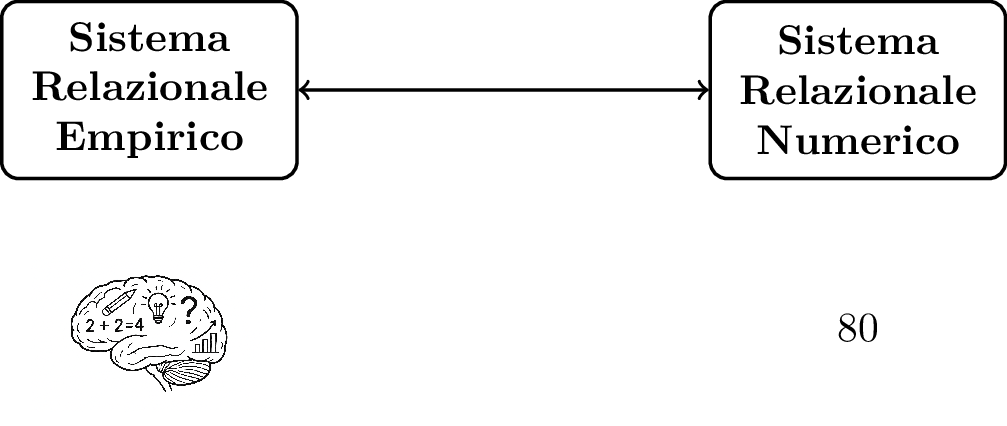
\includegraphics[width=0.7\linewidth,height=\textheight,keepaspectratio]{chapters/../Figures/Latex - Figure Measurement 2/Fig_measurement_2.png}
\end{center}

In questo caso possiamo dire che il nostro Sistema Relazionale
Empirico\footnote{è importante notare che non tutti sarebbero daccordo
  nel dire che l'insieme di costrutti psicologici (cioè concetti non
  osservabili) sono parte di un sistema relazionale empirico. La domanda
  è però proprio al confine dell'epistemologia: un concetto psicologico
  non osservabile è parte del mondo empirico (così come lo sono altri
  entità non osservabili) oppure no? Non è lo scopo di questo libro né
  di questo paragrafo rispondere a questa domanda, ma per i nostri scopi
  la diversa collocazione dei concetti psicologici (come entità del
  mondo empirico o no), è irrilevante. Qui assumo che i concetti
  psicologici siano di fatti parte dei sistemi relazionali empirici in
  un certo senso aggirando il problema, e utilizzando la definizione di
  sistema relazionale empirico come ogni sistema relazionale \emph{non}
  numerico.} è dato dall'insieme di tutte le persone con diversa memoria
e il Sistema Relazione Numerico come l'insieme di numeri che utilizziamo
per descrivere la memoria di queste persone. Alcune operazioni con
questi numeri sono intuitivamente sensate, ad esempio possiamo dire che
alcune persone hanno più memoria di altre (possiamo quindi ordinare), ma
nel momento in cui cerchiamo di capire l'applicabilità di altre
operazioni diventa più difficile rispondere. Ad esempio, tramite un test
possiamo arrivare a dire che una persona ha il doppio di memoria di un
altra? Oppure che ha +20 unità di memoria più di un'altra? (qualsiasi
sia questa unità). Per poter una risposta a queste domande, dovremmo
sapere appunto in che scala di misurazione è stata misurata la memoria.

Come sarà più volte ribadito, senza che sia esplicitamente detto,
\textbf{nella maggior parte dei test neuropsicologici \emph{si assume}
che la misura sia su una scala a intervalli}. Assumere una scala ad
intervalli indica che le differenze tra punteggi hanno un significato e
sono consistenti lungo tutta la scala. Questo ad esempio è intuitivo
quando si considera il classico esempio di scala ad intervalli, una
misura di temperatura (ad esempio in Celsius). Un aumento di 2 gradi
Celsius significa lo stesso aumento di gradi indipendentemente dallo
stesso valore di partenza: che questi si aggiungano a 38 o 40 gradi
(ottenendo quindi rispettivamente 40 e 42) o un qualsiasi altro valore
di partenza, in tutti i casi sono stati aggiunti 2 gradi Celsius.
Provare ad applicare lo stesso ragionamento su un test neuropsicologico
può non sembrare così naturale. Ad esempio aggiungere 2 punti al MoCA
dovrebbe avere lo stesso significato sia che si parta da 20 o che si
parta da 28. Ma possiamo veramente dire che un aumento di 2 punti al
MoCA ha sempre lo stesso significato? Un aumento da 26 a 28 indica una
prestazione medio-alta che diventa ancora più alta. Un aumento da 28 a
30 porta da una prestazione piuttosto alta ad una prestazione
perfetta\footnote{per complicare ulteriormente il quadro qualcuno che
  conosce il MoCA potrebbe anche dire che il significato di questi
  \(+2\), dipende molto da quale è l'item (o gli item) a cui è legato
  questo punteggio, questo esempio è trattato in un
  \hyperref[Approfondimento-item-arbitrari]{Approfondimento}).}. Un
altro esempio può essere fatto con un altro test come il Digit Span, in
cui viene chiesto di ricordare delle sequenze di numeri di lunghezza
crescente e il punteggio finale è dato dalla sequenza più lunga che si è
in grado di ricordare. Torniamo al nostro ipotetico esempio di un
aumento di 2 punti. Un aumento da 3 a 5, significa il passaggio dal
ricordare una sequenza veramente bassa ad una sequenza piuttosto alta.
Un aumento da 8 a 10 invece da una prestazione già molto alta ad una
prestazione eccezionale (provate a ricordarvi una sequenza di 8 o 10
numeri per rendervi conto di quanto è difficile). Queste considerazioni
sollevano già un primo problema: utilizzare i punteggi ``grezzi'' che si
ottengono da un test e interpretarli come in una scala ad intervalli,
sembra quantomeno problematico.

Si potrebbe pensare che questo problema è risolto nel momento in cui i
punteggi si ``standardizzano'' oppure si riconducono alla percentuale di
persone che ottengono quel punteggio nella popolazione (questo sarà il
tema principale del Capitolo 3), ma purtroppo per la maggior parte dei

Ricapitolando, significa assumere che gli intervalli tra punteggi
abbiano sempre lo stesso significato e questo sembra

Chi ha già utilizzato in ambito clinico dei test neuropsicologici
potrebbe pensare che quanto appena in realtà è un problema di scarsa
rilevanza quando si utilizzano i test solo per definire se c'è un
deficit o meno (quindi se il punteggio è al di sotto di una soglia). In
questo caso infatti, non facciamo operazioni come sottrazioni o
addizioni, ma semplicemente confrontiamo il nostro punteggio con un
altro e se inferiore allora inferiamo che ci potrebbe essere un deficit
(questo argomento sarà trattato in grande dettaglio nel
\hyperref[Capitolo2]{Capitolo 2}. In realtà ci sono altri aspetti in cui
potrebbero essere utilizzate delle operazioni che poi di fatto assumono
scala di intervalli. Un esempio è l'utilizzo di ``correzioni'' per età e
scolarità (che sono trattate nel capitolo 2 e nell'approfondimento sulle
regressioni). Un test che faccia utilizzo di griglie di correzioni quasi
inevitabilmente fa le assunzioni (non banali), che abbiamo appena
discusso e cioè che la misurazione avvenga in una scala ad intervalli.
Il perché di questo è anche facile da intuire perché le correzioni
spesso sono addizioni o sottrazioni al punteggio osservato per
\emph{correggere} il punteggio (e addizioni o sottrazioni sono
operazioni che hanno senso nella scala ad intervalli).

Si misurano concetti psicologici (o proprietà di concetti psicologici),
lo si fa tramite costrutti osservabili.

Questa domanda, anche se apparentemente semplice, apre una sorta di
``vaso di pandora'' nell'ambito della neuropsicologia e lo anticipo
subito, non riusciremo probabilmente a dare una risposta convincente, ma
solo a presentare una serie di riflessioni che è utile tenere a mente.

Tutte queste considerazioni sono assolutamente sensate (e comuni), ma
nell'ambito di una misurazione sono semplicemente basate sul buon senso
e non basate su un modello di misurazione. Il neuropsicologo dovrebbe
conoscere questi aspetti per capire meglio e anche per scegliere in
maniera più consapevole. Alcuni test neuropsicologici infatti non
soffrono di questi problemi perché sviluppati in maniera in cui il
significato delle variazioni di punteggio è molto più preciso. Questi
test sono sviluppati secondo altri modelli di misurazione (ad esempio la
famiglia di modelli nota come Item Response Theory). Purtroppo però, per
una serie di ragioni, probabilmente pratiche e storiche, i test
neuropsicologici che hanno queste caratteristiche sono veramente pochi e
quindi dobbiamo accontentarci di sturmenti di misura in cui \emph{si
assume} con tutte le problematicità evidenziate, una scala ad
intervalli.

\textbf{DA RIVEDERE QUI NON SI INCASTRA BENE LA FRASE} Come sarà ripreso
nel paragrafo
\hyperref[introduzione-item-response-theory]{\emph{Introduzione all'Item
Response Theory}}) e nel capitolo
\hyperref[misurare_cambiamenti]{\emph{Misurare Cambiamenti nel Tempo}},
questa è un'assunzione che potrebbe non essere rispettata, e alcune
delle conseguenze di questa assunzione richiedono una riflessione sulle
sue implicazioni.

Ricapitolando questo paragrafo, XXXXXXXX Vorrei chiarire che il
neuropsicologo (clinico o forense), non dovrebbe porsi quotidianamente
il problema sulla scala di misurazione del test che sta usando, a meno
che non decida di fare delle operazioni sui punteggi che non sono quelle
normalmente previste per la pratica clinica e dal test stesso. Il
messaggio importante è: \textbf{il fatto che abbiamo ottenuto dei numeri
non ci permette di fare ciò che vogliamo di questi numeri}. Alcune
operazioni, anche se praticamente possibili, possono essere delicate o
problematiche e sapere che esse sono la conseguenza di una semplice
assunzione (discutibile per certi aspetti), è importante per una
corretta interpretazione dei punteggi.

\section{I test}\label{i-test}

Già dall'introduzione è stato detto che il protoganista assoluto del
libro è il test neuropsicologico. Ma cosa è un test? Come sempre, non
possiamo non procedere senza fornire una definizione precisa che ci
aiuti a definire cosa è un test (e cosa non lo è) e quali sono le
caratteristiche che lo contraddistinguono.

\begin{itemize}
\tightlist
\item
  Esistenza di tante definizioni
\item
  Definizione di Test di Cronbach (con limite)
\item
  Definizione di Test di Chiorri
\item
  Figura adattata da Methodology su relazione tra punteggio e costrutto.
\item
  Citazione Lezak (su limiti test e misurazione costrutti)
\end{itemize}

\subsection{Test di prestazione
tipica}\label{test-di-prestazione-tipica}

\subsection{Test di prestazione
massima}\label{test-di-prestazione-massima}

\subsection{Alti test utili per la valutazione
neuropsicologica}\label{alti-test-utili-per-la-valutazione-neuropsicologica}

(Es. test di stima di riserva Criq, scale IADL ADL, etc.)

\section{Teoria Classica dei test}\label{teoria-classica-dei-test}

\section{Validità ed Affidabilità}\label{validituxe0-ed-affidabilituxe0}

\subsection{Tipi di Validità e perché sono
importanti}\label{tipi-di-validituxe0-e-perchuxe9-sono-importanti}

\subsubsection{Validità di costrutto}\label{validituxe0-di-costrutto}

\subsubsection{Validità concorrente}\label{validituxe0-concorrente}

\subsubsection{Validità predittiva}\label{validituxe0-predittiva}

\subsubsection{Validità interna}\label{validituxe0-interna}

\subsubsection{Validità di facciata}\label{validituxe0-di-facciata}

\subsubsection{Validità ecologica}\label{validituxe0-ecologica}

\section{Affidabilità}\label{affidabilituxe0}

\subsection{Tipi di affidabilità e perché sono
importanti}\label{tipi-di-affidabilituxe0-e-perchuxe9-sono-importanti}

\subsubsection{Consistenza Interna}\label{consistenza-interna}

\subsubsection{Affidabilità Test
Retest}\label{affidabilituxe0-test-retest}

\subsubsection{Affidabilità
Split-Half}\label{affidabilituxe0-split-half}

\subsubsection{Inter-Rater Agreement}\label{inter-rater-agreement}

\section{Introduzione alla Item Response
Theory}\label{introduzione-item-response-theory}

\section{Nella pratica clinica: Come usare Affidabilità e Validità per
scegliere i
test}\label{nella-pratica-clinica-come-usare-affidabilituxe0-e-validituxe0-per-scegliere-i-test}

\section{Nella pratica clinica: Come usare Affidabilità e Validità per
interpretare i
test}\label{nella-pratica-clinica-come-usare-affidabilituxe0-e-validituxe0-per-interpretare-i-test}

\section{Errori comuni nel considerare gli aspetti psicometrici dei
test.}\label{errori-comuni-nel-considerare-gli-aspetti-psicometrici-dei-test.}

\bookmarksetup{startatroot}

\chapter*{Bibliografia}\label{bibliografia}
\addcontentsline{toc}{chapter}{Bibliografia}

\markboth{Bibliografia}{Bibliografia}

\printbibliography[heading=none]

\bookmarksetup{startatroot}

\chapter*{Lavoro in fase di sviluppo}\label{lavoro-in-fase-di-sviluppo}
\addcontentsline{toc}{chapter}{Lavoro in fase di sviluppo}

\markboth{Lavoro in fase di sviluppo}{Lavoro in fase di sviluppo}

\begin{center}{\Large \textcolor{gray}{\textbf{Questo Libro è ancora in fase di scrittura,\\ per versioni aggiornate visita il sito\\ \url{giorgioarcara.github.io/oip-book} e la newsletter del libro \url{oltreipunteggi.substack.com/}}}} \end{center}

\part{Appendici}

\chapter*{A1. Note di redazione}\label{note_redazione}
\addcontentsline{toc}{chapter}{A1. Note di redazione}

\markboth{A1. Note di redazione}{A1. Note di redazione}

\subsection*{Un libro Open}\label{un-libro-open}
\addcontentsline{toc}{subsection}{Un libro Open}

La decisione di scrivere un libro \emph{Open} (cioè liberamente
scaricabile, modificabile e riutilizzabile) è innanzitutto una scelta
ideologica: sono un convinto sostenitore dell'Open Science da oltre
quindici anni e ritengo che, per un testo di questo tipo, sia l'opzione
più logica. Gran parte dei libri e delle risorse da cui ho appreso i
contenuti che propongo in queste pagine erano, o sono tuttora,
liberamente accessibili, e considero questa modalità non solo sensata,
ma anche eticamente corretta. Oltre alla dimensione ideologica, un libro
\emph{Open} come questo offre ulteriori vantaggi, che verranno
illustrati nel paragrafo seguente.

\subsection*{Un libro collaborativo}\label{un-libro-collaborativo}
\addcontentsline{toc}{subsection}{Un libro collaborativo}

Il libro è pensato per essere scritto anche contando sul contributo dei
lettori. I contributi possono essere segnalazioni di typos, richiesta di
chiarimenti, o di approfondimento, ma sono anche apprezzati anche
commenti generali (es. suggerimenti a rimodulare la struttura di un
capitolo). Non escludo di includere anche intere sezioni scritte da
altre persone, se vorranno contribuire in questa maniera. Ovviamente, se
il contributo sarà sostanziale, la persona sarà inserita tra coautori
del libro. Alla destra di ogni pagina trovi due pulsanti che aiutano per
una comunicazione rapida. Nota che per utilizzarli dovrai però creare un
account \texttt{github}:

\begin{itemize}
\tightlist
\item
  \emph{``Segnala un problema''} può essere utilizzato per segnalare un
  errore generale o se vuoi lasciarmi un commento esteso.
\item
  \emph{``Modifica questa pagina''} , può essere utilizzato se vuoi dare
  un contributo più fattivo e direttamente suggerire una correzione.
  Queste mi verranno segnalato e potrò incorporarle. Puoi utilizzare
  questo strumento per piccole modifiche, ma se pensi di fare una
  modifica sostanziale ti chiedo di contattarmi prima e di concordarla.
  Questo è per rispetto del tuo tempo, nel caso alla fine preferissi non
  inserire la modifica.
\end{itemize}

In alternativa a questi, considera sempre che puoi scrivermi una mail a
\href{mailto:giorgio.arcara@gmail.com}{\nolinkurl{giorgio.arcara@gmail.com}}.
Se sei pratico di github ovviamente sei invitato ad utilizzarlo, creando
una fork e poi aprendo pull request per le modifiche. Ricorda che
contribuendo accetti che i tuoi testi vengano inclusi sotto la licenza
del progetto (CC BY-NC-SA 4.0).

\subsection*{Un libro in costante
miglioramento}\label{un-libro-in-costante-miglioramento}
\addcontentsline{toc}{subsection}{Un libro in costante miglioramento}

Ho scelto di scrivere un libro in questa modalità, tramite un sito e un
.pdf scaricabile associato, perché sono fermamente convinto che (nel
2025, momento in cui sto cominciando a scrivere il volume), bisogna
sfruttare tutte le opportunità date dalla tecnologia. Psicometria e
statistica applicate alla neuropsicologia sono anche discipline in
costante crescita e un libro pubblicato tramite canali tradizionali
rischierebbe di essere obsoleto in alcune sue parti già al momento della
pubblicazione. Usare questo sistema permetterà anche un miglioramento
dopo che il libro potrà essere considerato completo. Il libro usa una
convenzione numerica ispirata al \textbf{Semantic Versioning (SemVer)}
(sistema di numerazione di versioni dei software), adattato al processo
di scrittura.

Il formato è:

\begin{verbatim}
vMAJOR.MINOR.PATCH[-fase]
\end{verbatim}

\subsubsection*{Significato delle parti}\label{significato-delle-parti}
\addcontentsline{toc}{subsubsection}{Significato delle parti}

\begin{itemize}
\tightlist
\item
  \textbf{MAJOR} → Cambia quando viene raggiunta una pietra miliare
  importante (es. bozza completa, revisione principale, versione
  finale).
\item
  \textbf{MINOR} → Cambia quando viene aggiunto un nuovo capitolo o una
  sezione importante, o quando avviene una ristrutturazione
  significativa del testo.
\item
  \textbf{PATCH} → Cambia per correzioni minori, refusi, aggiustamenti
  di frasi, formattazione.
\end{itemize}

\subsubsection*{Etichette di fase}\label{etichette-di-fase}
\addcontentsline{toc}{subsubsection}{Etichette di fase}

\begin{itemize}
\tightlist
\item
  \textbf{alpha} → Bozza iniziale, non revisionata.
\item
  \textbf{beta} → Contenuti quasi completi, pronti per revisione.
\item
  \textbf{rc} (release candidate) → Testo completo e rivisto, in attesa
  di pubblicazione.
\item
  \emph{Nessuna etichetta} → Versione finale.
\end{itemize}

\subsubsection*{Esempi}\label{esempi}
\addcontentsline{toc}{subsubsection}{Esempi}

\begin{verbatim}
v0.1.0-alpha   # Primo capitolo in bozza
v0.1.1-alpha   # Piccole correzioni al primo capitolo
v0.2.0-alpha   # Secondo capitolo in bozza
v1.0.0-beta    # Bozza del libro completa, in revisione
v1.0.0         # Prima Versione finale pubblicata
\end{verbatim}

Nota che la numerazione inizia da \textbf{0} finché il libro non è
completo.

\subsection*{Una nota sul titolo}\label{una-nota-sul-titolo}
\addcontentsline{toc}{subsection}{Una nota sul titolo}

Il titolo del libro, \emph{Oltre i punteggi}, è volto a sottolineare la
mia posizione sull'importanza di integrare i punteggi ai test con altre
informazioni e non penso abbia bisogno di altre spiegazioni. Il
sottitolo del libro invece sottolinea che tratterà di due aspetti,
psicometria e statistica, strettamente legati ma che è utile non
confondere. L'utilizzo dei test neuropsicologici infatti è spesso
(specie in Italia) concentrato molto sulla cura degli aspetti
\emph{statistici} (e in particolare associati a probabilità di ottenere
certi punteggi) ma meno su quelli \emph{psicometrici} e cioè su quanto
accurate sono le nostre misurazioni e su quanto i punteggi che abbiamo
ottenuti siano effettivamente rappresentativi di ciò che ci interessa
(es. il funzionamento cognitivo).

\subsection*{Femminile e maschile nel
testo}\label{femminile-e-maschile-nel-testo}
\addcontentsline{toc}{subsection}{Femminile e maschile nel testo}

In un ottica di gender balance ho deciso di evitare il più possibile di
usare solo il maschile nel testo mettendo ogni volta che fosse
necessario prima femminile e poi maschile (es. la/il neuropsicologa/o).
Questa è una scelta che ho dovuto inevitabilmente fare visto che la
prima stesura del testo è in Italiano. Mi rendo conto che questa scelta,
per quanto motivata, potrebbe rendere più difficile la lettura. Le
evidenze sull'impatto di una scelta come questa nella lettura sono
tuttora non chiare e mi sono basato quindi su un criterio più personale
che non su evidenze scientifiche.

\subsection*{Utilizzo di AI nella stesura del
libro}\label{utilizzo-di-ai-nella-stesura-del-libro}
\addcontentsline{toc}{subsection}{Utilizzo di AI nella stesura del
libro}

Nel momento in cui sto cominciando a scrivere questo libro (Agosto
2025), siamo in piena esplosione dell'utilizzo e delle opportunità di
sistemi di Intelligenza Artificiale (In particolare Large Language
Models, LLM come ChatGPT). Sta diventando sempre più comune dunque
esplicitare che utilizzo se ne è fatto, in maniera trasparente. Tutte le
idee di questo libro sono generate \textbf{senza} l'ausilio di sistemi
di intelligenza artificiale. Sistemi di AI (e in particolare ChatGPT)
sono stati utilizzati per i seguenti scopi:

\begin{itemize}
\tightlist
\item
  revisione del testo (per typos o miglioramento chiarezza di alcune
  frasi)
\item
  supporto nel codice per generare il libro (Quarto e i linguaggi
  associati).
\item
  generazioni di alcune immagini esemplificative o per l'immagine di
  copertina (questo per evitare problemi di immagini con copyright).
\item
  supporto nella generazione di codice \texttt{R} per alcuni esempi.
\end{itemize}

In ogni caso, mi prendo ogni responsabilità di errori legati
all'utilizzo di sistemi di AI.

\chapter*{A2. Registro aggiornamenti}\label{registro_aggiornamenti}
\addcontentsline{toc}{chapter}{A2. Registro aggiornamenti}

\markboth{A2. Registro aggiornamenti}{A2. Registro aggiornamenti}

\subsection*{v0.0.1 - 5/09/2025}\label{v0.0.1---5092025}
\addcontentsline{toc}{subsection}{v0.0.1 - 5/09/2025}

Rilasciata versione iniziale del libro che include

\begin{itemize}
\tightlist
\item
  Premesse
\item
  Introduzione
\item
  Appendici A1 e A2
\end{itemize}

\subsection*{\texorpdfstring{v0.1.0 - \emph{in
corso}}{v0.1.0 - in corso}}\label{v0.1.0---in-corso}
\addcontentsline{toc}{subsection}{v0.1.0 - \emph{in corso}}

\begin{itemize}
\tightlist
\item
  corretti vari typos e migliorato il flusso di alcune frasi.
\item
  aggiunta quarta di copertina.
\item
  aggiunta prima versione del Capitolo 1.
\item
  aggiunta previsione di nuovi paragrafi (Riassunti a fine capitolo e
  paragrafo su AI).
\end{itemize}

\chapter*{A3. Definizioni}\label{note_redazione}
\addcontentsline{toc}{chapter}{A3. Definizioni}

\markboth{A3. Definizioni}{A3. Definizioni}

\subsection*{Perché sono importanti le
definizioni.}\label{perchuxe9-sono-importanti-le-definizioni.}
\addcontentsline{toc}{subsection}{Perché sono importanti le
definizioni.}

Un libro che ambisce a insegnare l'importanza della metodologia non può
prescindere dall'includere una sezione con le definizioni dei termini
più importanti. Questo è fondamentale perchè le definizioni di termini
anche comunemente usati in neuropsicologia o nell'uso dei test, come
\emph{``normalità''} ha un impatto enorme nei metodi che poi usiamo.

\subsubsection*{Psicometria}\label{psicometria}
\addcontentsline{toc}{subsubsection}{Psicometria}

La Psicometria è quella disciplina che studia teorie e metodi di
misurazione in psicologia. Nello specifico si occupa di test,
misurazioni e valutazioni di tipo psicologico e di misurazione di
costrutti latenti (cioè non osservabili).
\href{https://en.wikipedia.org/w/index.php?title=Psychometrics&oldid=1307897603}{fonte:
Wikpedia}

\emph{Nota}: la psicometria fa grande utilizzo di metodi di statistica,
tanto che, specie in ambito psicologico, spesso c'è confusione tra i
confini tra le due discipline. Anche se è vero che ci sono numerose aree
di sovrapposizione (perché la Psicometria fa utilizzo di tecniche
statistiche), non sono da considerare come sinonimi, visto che molti
aspetti psicometrici non sono strettamente statistici e numerosi aspetti
statistici non è detto che siano rilevanti per la psicometria.

\subsubsection*{Statistica}\label{statistica}
\addcontentsline{toc}{subsubsection}{Statistica}

La statistica è quella disciplina che studia la raccolta, descrizione,
analisi e interpretazione di \emph{dati}, La statistica si occupa di
ogni fase del trattamento dei dati, dalla pianificazione dei disegni,
fino alle tecniche di analisi e inferenze sui risultati ottenuti.
\href{https://en.wikipedia.org/w/index.php?title=Statistics&oldid=1307451692}{fonte:
Wikpedia}

\emph{Nota}: è importante conoscere la statistica non solo perché essa
viene utilizzata abbondantemente in psicometria, ma anche perché certi
aspetti rilevanti per le interpretazioni di test neuropsicologici sono
meramente statistici (e non psicometrici, secondo la definizione di
``psicometria'' riportata sopra). Ad esempio stimare le probabilità di
classificare un paziente come a rischio di Alzheimer a partire da dati
biologici e anamnestici non prevede misurazioni di costrutti psicologici
e quindi non è pertinenza delle psicometria.

\subsubsection*{Valutazione
neuropsicologica}\label{valutazione-neuropsicologica}
\addcontentsline{toc}{subsubsection}{Valutazione neuropsicologica}

La valutazione neuropsicologica è un esame clinico in cui si cerca di
ottenere informazioni sullo stato cognitivo di un individuo a fini
diagnostici, prognostici o riabilitativi. Essa consiste in genere in
raccolta di dati anamnestici, un colloquio e la somministrazione di test
standardizzati. Tutte queste informazioni sono integrate per stilare un
referto neuropsicologico.


\backmatter

\clearpage
\ifodd\value{page}\hbox{}\newpage\fi
% Insert the back cover PDF, full page
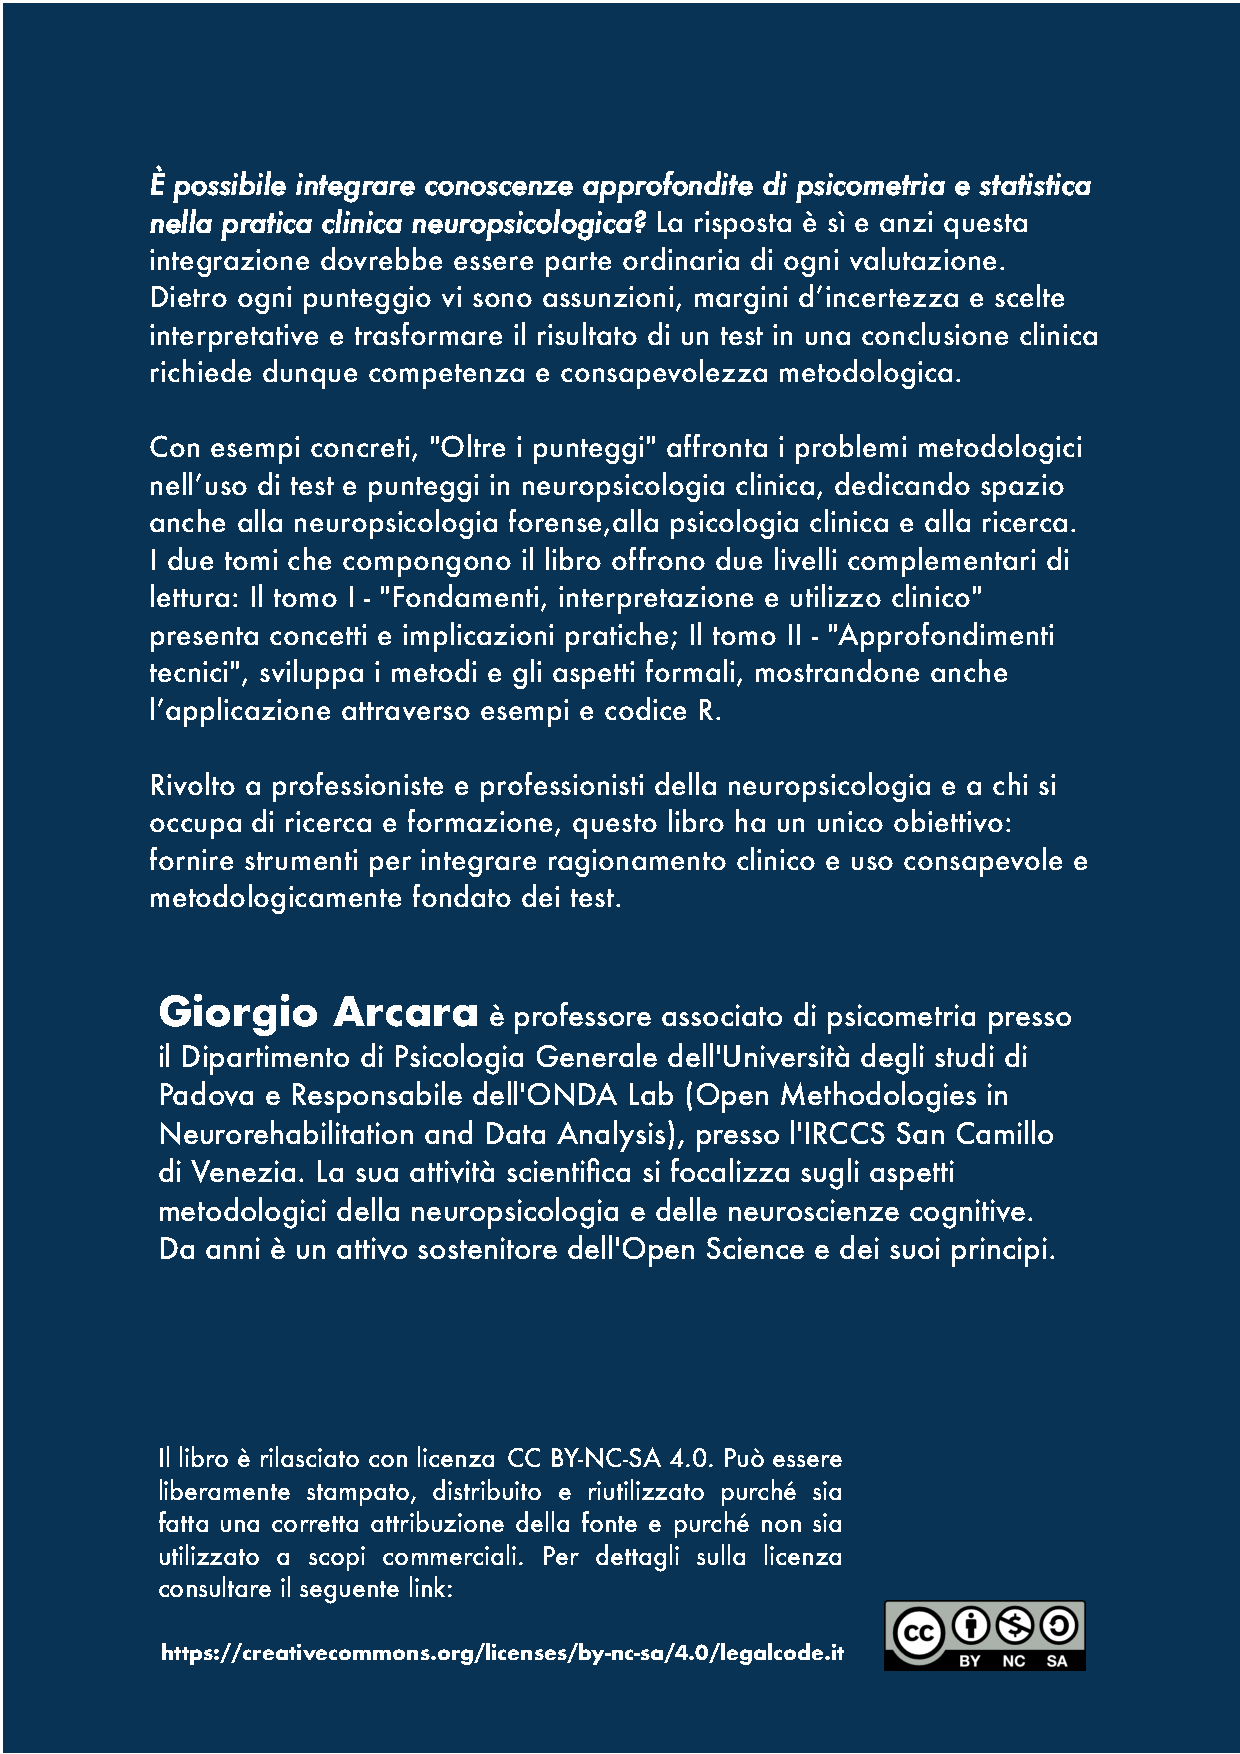
\includepdf[pages=-,fitpaper]{Figures/Quarta.pdf}
%\begin{center}
%{\Large
%\textit{Questo è un libro in fase di scrittura.}\\
%Per aggiornamenti visita: \url{https://giorgioarcara.github.io/oip-book}\\
%Ultimo rendering: \today\  \currenttime
%}
%\end{center}
%\setkomafont{section}{\headingfont\bfseries\Large}
%\setkomafont{subsection}{\headingfont\bfseries\large}
%\printbibliography


\end{document}
